\documentclass[9pt]{beamer}

\usepackage[T1]{fontenc}
\usepackage{color}
\usepackage{graphicx}
\usepackage{natbib}
\usepackage{tikz}

\usepackage{tcolorbox}

\usetheme{Boadilla}

\usefonttheme{professionalfonts}

\title[Apsis Tools]{Computational Tools to Understand and Support the Science Policy Interface in the Age of Big Literature: The Case of Climate Policy}
\subtitle{}
\author{Max Callaghan}
\institute[MCC]{
	%
\includegraphics[height=1cm,width=2cm]{/home/max/Pictures/MCC_Logo_RZ_rgb.jpg}
	
\includegraphics[height=1cm,width=2cm]{MCC_Logo_RZ_rgb.jpg}
}


\newtheorem*{remark}{}

\bibliographystyle{apalike}

\begin{document}
	
\begin{frame}
	\titlepage
\end{frame}

\addtobeamertemplate{frametitle}{}{%
	\begin{tikzpicture}[remember picture,overlay]
	\node[anchor=north east,yshift=2pt] at (current page.north east) {
\includegraphics[height=0.8cm]{MCC_Logo_RZ_rgb.jpg}};
	\end{tikzpicture}}

\begin{frame}{Motivation}

\begin{columns}
	\begin{column}{0.5\linewidth}<1->
		\begin{center}
			\begin{figure}
				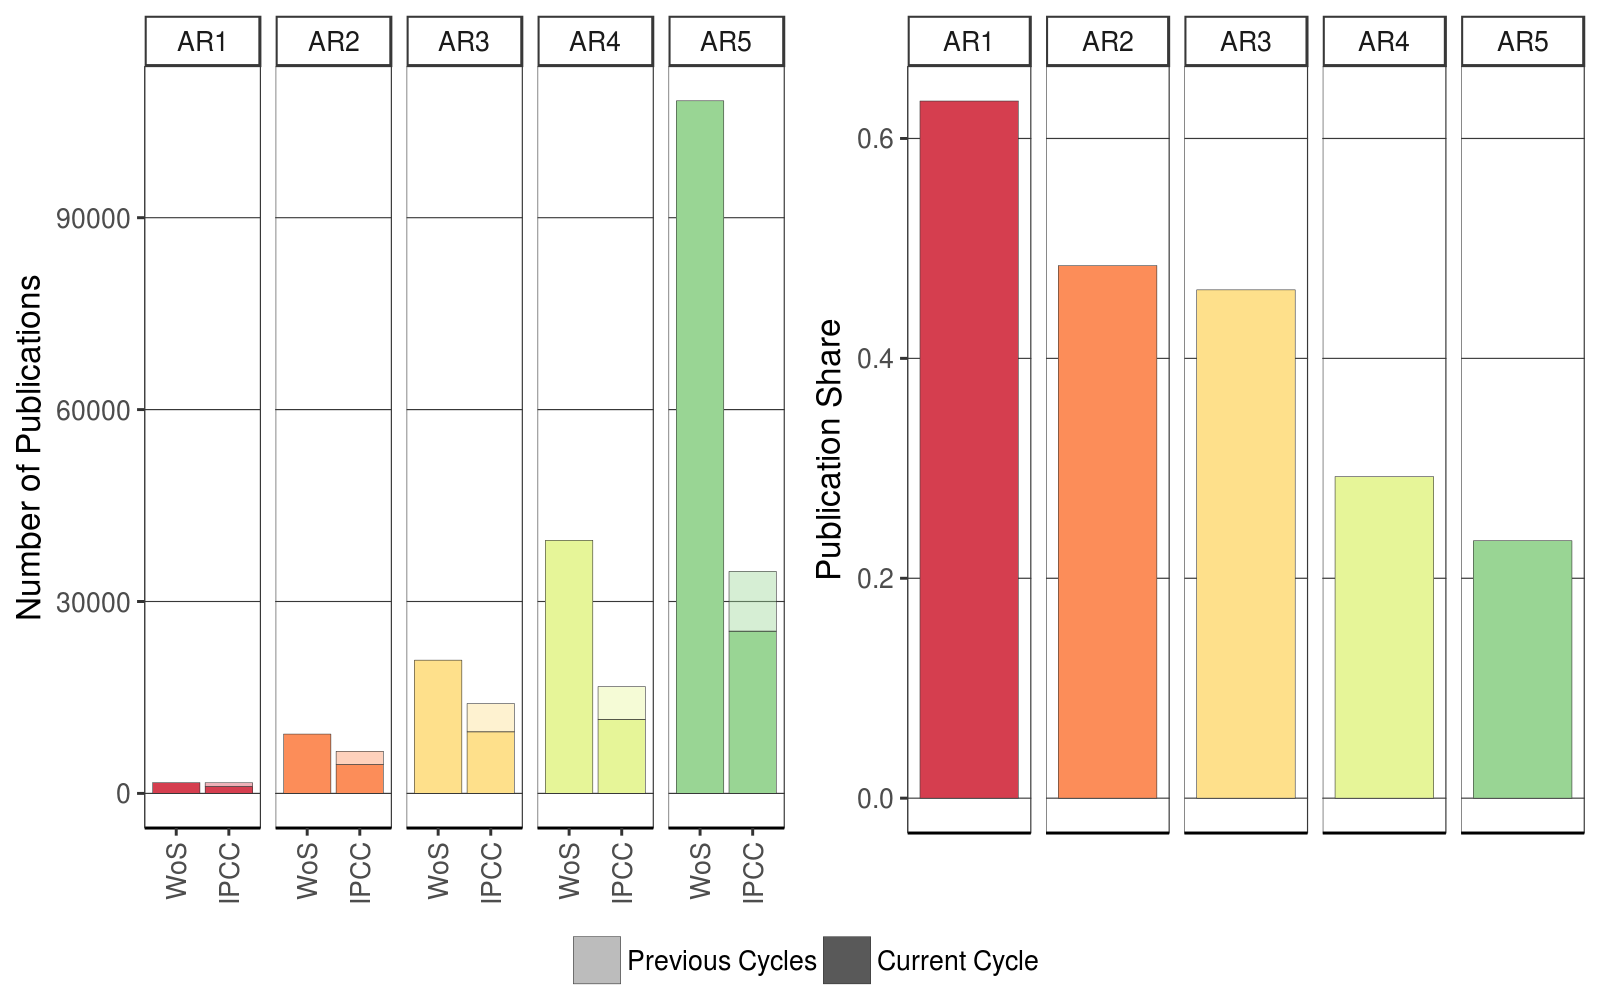
\includegraphics[width=0.85\linewidth]{images/merged_IPCC_spectral.png}
				\caption{Source: \citep{Minx2017l}}
				
			\end{figure}
		\end{center}
	\end{column}
	\begin{column}{0.5\linewidth}<2>
		\begin{center}
			\begin{figure}
				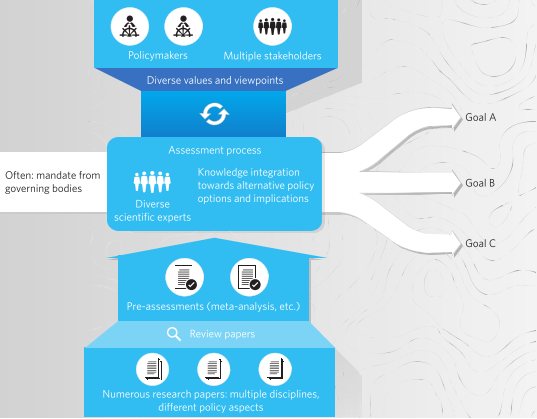
\includegraphics[width=0.85\linewidth]{images/pyramid.png}
				\caption{Source: \citep{Kowarsch2015}}
			\end{figure}
		\end{center}
	\end{column}
\end{columns}

\end{frame}

\begin{frame}{Approach}
To answer quantitatively:
\begin{itemize}
	\item What do the layers of the pyramid look like?
	\item How does information flow between them?
\end{itemize}

\begin{columns}
	\begin{column}{0.5\linewidth}
		\scriptsize
	\begin{figure}
		\begin{tcolorbox}[colback=green!5,colframe=green!40!black,title=Mapping Climate Change Knowledge, boxsep=2pt,left=4pt,right=4pt,top=2pt,bottom=2pt, enlarge bottom by=-0.25cm, enlarge top by=-0.25cm]
			\noindent
			What is the relevant literature, what does the landscape look like?
		\end{tcolorbox}
	\end{figure}
	
		\begin{figure}
			\begin{tcolorbox}[colback=green!5,colframe=green!40!black,title=Big Literature in Climate Change, boxsep=2pt,left=4pt,right=4pt,top=2pt,bottom=2pt, enlarge bottom by=-0.25cm, enlarge top by=-0.25cm]
				\noindent
				How `Big' (in volume, variety and velocity) is Climate Change Literature
			\end{tcolorbox}
		\end{figure}
		
		\begin{figure}
			\begin{tcolorbox}[colback=green!5,colframe=green!40!black,title=Knowledge Accumulation and Blind Spots, boxsep=2pt,left=4pt,right=4pt,top=2pt,bottom=2pt, enlarge bottom by=-0.25cm, enlarge top by=-0.25cm]
				\noindent
				Compare IPCC with references and wider literature to assess coverage and knowledge accumulation
			\end{tcolorbox}
		\end{figure}
		
	\begin{figure}
		\begin{tcolorbox}[colback=green!5,colframe=green!40!black,title=Evidence in Policymaking, boxsep=2pt,left=4pt,right=4pt,top=2pt,bottom=2pt, enlarge bottom by=-0.25cm, enlarge top by=-0.25cm]
			\noindent
			What types of evidence gets used in different fields of policymaking?
		\end{tcolorbox}
		
	\end{figure}
	
	\end{column}
	\begin{column}{0.5\linewidth}
		\begin{center}
			\begin{figure}
				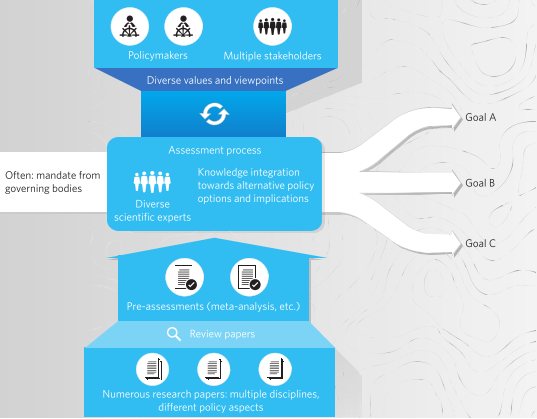
\includegraphics[width=0.85\linewidth]{images/pyramid.png}
			\end{figure}
		\end{center}
	\end{column}
\end{columns}

\end{frame}



\begin{frame}{Frame Title}
	\small
	%\bibliography{/home/max/Documents/library/bibliography}
	\bibliography{C:/Users/galm/Documents/library/library}
\end{frame}

\end{document}
